\section{Mechanische Arbeit, Energie und Leistung}
\subsection{Arbeit}
Wirkt eine Kraft entlang eines Weges, so wird im physikalischen Sinn \textbf{mechanische Arbeit} geleistet. Die Arbeit hat die Einheiten [W]=Nm=Joule. Nur die Komponente der Kraft in Richtung des Weges leistet Arbeit. Für $90^{\circ}<\varphi<270^{\circ}$ ist die Arbeit negativ und in diesem Fall ist die Aerbeit verrichtete Komponente der Kraft entgegengesetzt gerichtet zum Weg. 
\begin{equation}
\boxed{
\begin{array}{lll}
W&=&\overrightarrow{F}\bullet \overrightarrow{s}\\
&=&\Big\vert \overrightarrow{F}\Big\vert\cdot \Big\vert \overrightarrow{s}\Big\vert\cdot \cos\left(\varphi\right)
\end{array}
}
\end{equation}
\begin{figure}[H]
\frame{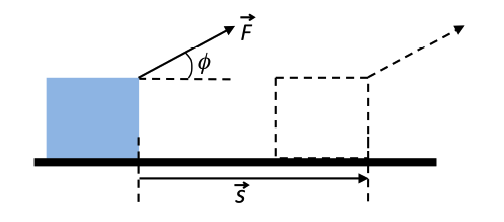
\includegraphics[scale=0.5]{../img/I/Ia}}
\centering
\caption{Mechanische Arbeit bei konstanter Kraft $\vec{F}$ über eine Verschiebung $\vec{s}$. Zur Arbeit trägt die zu $\vec{s}$ antiparallele Komponente $F\cdot \cos\left(\varphi\right)$}
\label{fig_Ia}
\end{figure}
\noindent Ist die Kraft abhängig von der Wegrichtung, kann die Arbeit $\text{d}W$ nur für infinitesimal kleine Verschiebungen $\text{d}s$ definiert werden. Die Arbeit ist die Fläche unter der Kurve. Die Zufuhr oder Entnahme von Arbeit verändert die Energie des Systems. \textbf{positive Arbeit:} Arbeit wird in das System hineingesteckt und die Energie des Systems wird erhöht. \textbf{negative Arbeit:} Das System leistet Arbeit und die Energie des Systems wird erniedrigt.
\begin{figure}[H]
\frame{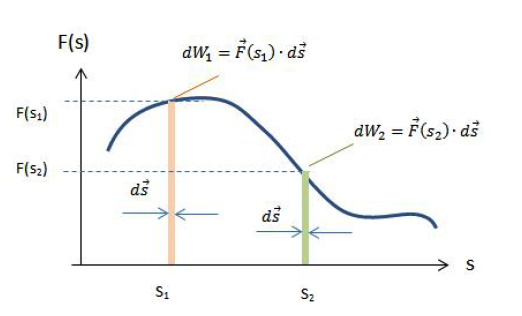
\includegraphics[scale=0.5]{../img/I/Ib}}
\centering
\caption{Da die Kraft im Allgemeinen wegabhängig ist, kann die Arbeit $\text{d}W$ nur für sehr kleine Verschiebungen d$s$ definiert werden.}
\label{fig_Ib}
\end{figure}   
\begin{equation}
\boxed{W_{12}=\displaystyle\int_{s1}^{s2}\overrightarrow{F}\left(\overrightarrow{s}\right)\bullet \text{d}\overrightarrow{s}}
\end{equation}
Energie und Arbeit haben die gleiche Einheit. Arbeit ist eine \textbf{Prozessgrösse} und ist abhängig vom Weg. Energie ist eine \textbf{Zustandsgrösse} und ist unabhängig vom Weg.
\subsection{Potentielle Energie}
Wird Arbeit geleistet um ein Körper gegen die Erdanziehung in die Höhe zu heben oder um eine Feder zu spannen, so ist die Arbeit nicht verloren. Diese Arbeit bleibt als Energie im Körper gespeichert und kann wieder verwendet werden, um Arbeit zu leisten. Diese Form gespeicherter Arbeit heisst \textbf{potentielle Energie}. 
\\\\
Wird ein Körper durch eine Kraft $\overrightarrow{F}_H$ gegen die äussere Gewichtskraft $\overrightarrow{F}_G=m\overrightarrow{g}$ um die Höhe $h$ angehoben, so wird dabei die Arbeit $W=mgh$ geleistet.
\begin{equation}
\boxed{E_{\text{pot}}=\Big\vert\overrightarrow{F}_G \Big\vert \cdot \Big\vert h\Big\vert = m\cdot \Big\vert \overrightarrow{g}\Big\vert\cdot \Big\vert h\Big\vert }
\end{equation}
\begin{figure}[H]
\frame{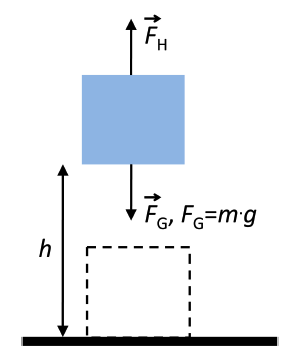
\includegraphics[scale=0.5]{../img/I/Ic}}
\centering
\caption{Beim Anheben eines Körpers gegen die Gravitationskraft wird Arbeit in Form von potentieller Energie gespeichert.}
\label{fig_Ic}
\end{figure} 
\subsection{Federenergie}
Wird eine Feder gespannt, so wird die in Feder gespeicherte Energie erhöht. Die gespeicherte potentielle Energie beträgt bei einem \textbf{linearen Feder}
\begin{equation}
\boxed{E_{\text{pot}}=\int_{0}^x\left(k\cdot x\right)\,\text{d}x}
\end{equation}
und bei einem \textbf{Torsionsfeder}
\begin{equation}
\boxed{E_{\text{pot}}=\int_{0}^x\left(k^{*}\cdot \varphi\right)\,\text{d}\varphi=\dfrac{1}{2}\cdot k^*\cdot \varphi^2}
\end{equation}
\subsection{Kinetische Energie}
Wird ein Körper beschleunigt, so wird Beschleunigungsarbeit geleistet. Seine \textbf{kinetische Energie} wird dabei erhöht. Die kinetische Energie für einen Körper, der sich mit Geschwindigkeit $v$ bewegt ist 
\begin{equation} 
\boxed{E_{\text{kin}}=\dfrac{1}{2}\cdot m\cdot \Big\vert \overrightarrow{v}\Big\vert^2}
\end{equation} 
Eine Kraft, die an einem Körper Arbeit leistet, führt zu einer Änderung der kinetischen Energie. \textbf{Positive Arbeit} $W>0$ führt zu einer Beschleunigung des Körpers, \textbf{negative Arbeit} $W<0$ bremst den Körper ab. Wird ein Körper beschleunigt, so speichert er die an ihm geleistete Arbeit in Form von kinetischer Energie. Er kann mit dieser Energie wieder Arbeit leisten.
\begin{equation}
\boxed{W=\triangle E_{\text{kin}}=\dfrac{1}{2}\cdot m\cdot \Big\vert \triangle\overrightarrow{v}\Big\vert^2=\dfrac{1}{2}\cdot m\cdot \left(v_e^2-v_a^2\right)} 
\end{equation} 
Für die kinetische Energie \textbf{rotierender Körpern} gilt folgende Beziehung, wobei $f$ die Drehzahl und $J$ das Massenträgheitsmoment sind
\begin{equation}
\boxed{E_{\text{kin}}=\dfrac{1}{2}\cdot J\cdot \left(2\pi\cdot f\right)^2}
\end{equation}
\subsection{Energieerhaltungssatz der Mechanik}
Energie kann weder verschwinden, noch aus dem Nichts erzeugt werden. Eine Energieform kann nur in eine andere Energieform umgewandelt werden. In einem \textbf{abgeschlossenen System} ist die Summe aller Energien konstant. Die Elemente können Energie untereinander austauschen, Energieformen können umgewandelt werden, aber die Gesamtenergie bleibt erhalten. 
\\\\
Ein physikalisches System ist eine Menge von Elementen, welche in Beziehung zueinander stehen und zwecks Untersuchung physikalischer Vorgänge durch eine Systemgrenze von der Umwelt getrennt werden. Man unterscheidet zwischen 
\begin{enumerate}
\item \textbf{Abgeschlossenes System:} Kein Austausch von Materie und Energie über die Systemgrenze. 
\item \textbf{Offenes System:} Systemgrenze ist durchlässig für Materie und Energie. 
\item \textbf{Geschlossenes System:} Kein Austausch von Materie, aber Systemgrenze ist durchlässig für Energie. 
\end{enumerate}
\subsection{Die Leistung}
In \textbf{offenen Systeme} findet ein Masse- und Energieaustausch über die Systemgrenze hinaus statt. Die Menge an Masse, bzw. Energie, die pro Zeiteinheit aufgenommen oder abgegeben wird ist der \textbf{Masse-} mit Einheit $\text{kg s}^{-1}$ und den \textbf{Energiestrom} mit Einheit $\text{J s}^{-1}=\text{Watt}$.
\begin{equation}
\boxed{\dot{m}=\dfrac{\triangle m}{\triangle t}}\quad 
\boxed{\dot{E}=\dfrac{\triangle E}{\triangle t}}
\end{equation}
Für das Vorzeichen von Energie- und Masseströme gilt die folgende Vorzeichenkonvenktion: Flüsse ins System $>0$, Flüsse aus dem System $<0$; d.h. die Zu- bzw. Abnahme von Masse und Energie in einem System wird immer vom System aus betrachtet.
\\\\
Der Energiestrom, also die Menge Energie welche pro Zeit in oder aus dem System fliesst, wird als \textbf{Leistung} $P$ bezeichnet und hat die Einheit [$P$]=Watt=Js$^{-1}$.
\begin{equation}
\boxed{P=\dfrac{\triangle E}{\triangle t}}
\end{equation}
\section{Wärme}
Wärme und Temperatur wird ständig verwechselt. Temperatur ist eine Zustandsgrösse, welche die innere Energie eines Körpers oder einer Substanz beschreibt. Wärme ist eine Form von Energie. Durch Reibungsarbeit konnte man die Temperaturdifferenzen messen. Wärme und mechanische Arbeit sind äquivalent.
\\\\
In einem Liter Wasser führt eine zugeführte Reibarbeit von 4187J zu einer Temperaturerhöhung von 1$^{\circ}$C. Dies nennt man das \textbf{mechanische Wärmeäquivalent}. Das war die Basis der veralteten Einheit Kalorie. Die Umwandlung von Wärme in Arbeit ist die Grundlage von Wasserkraftmaschinen wie Automotoren oder Dampfturbinen und somit Basis für die Industriegesellschaft. Die Wärme ist eine Energieform durch deren Zufuhr bzw. Abfuhr die kinetische Energie der Teilchen erhöht bzw. reduziert werden kann.
\subsection{Die Temperatur}
Dei Temperatur ist ein Mass für die thermische Bewegung der Teilchen. Ein einzelnes Teilchen besitzt keine Temperatur. Werden ein warmer und ein kalter Gegenstand miteinander in Kontakt gebracht, so wird Wärmeenergie vom wärmeren auf den kälteren Körper übertragen. Die kinetische Energie der Teilchen wird übertragen. Haben beide Körper die gleiche Temperatur, so findet keine Wärmeenergieübertragung statt. Die Gegenstände befinden sich im \textbf{thermischen Gleichgewicht}.
\\\\
In Europa wird die Temperatur mit Celsius Skala $[\theta]=^{\circ}$C während in den USA die Fahrenheit Skala $[\theta]=^{\circ}$F gemessen. In der Wissenschaft wird die Kelvinskala $[\theta]=^{\circ}$K verwendet mit absoluten Nullpunkt bei $-273.15^{\circ}$C. 
\begin{equation}
\boxed{\theta(^{\circ}F)=1.8\cdot \theta(^{\circ}C)+32}
\end{equation}
\begin{equation}
\boxed{\theta(^{\circ}K)=\theta(^{\circ}C)+273.15}
\end{equation}
\subsection{Die thermische Ausdehnung}
\begin{figure}[H]
\frame{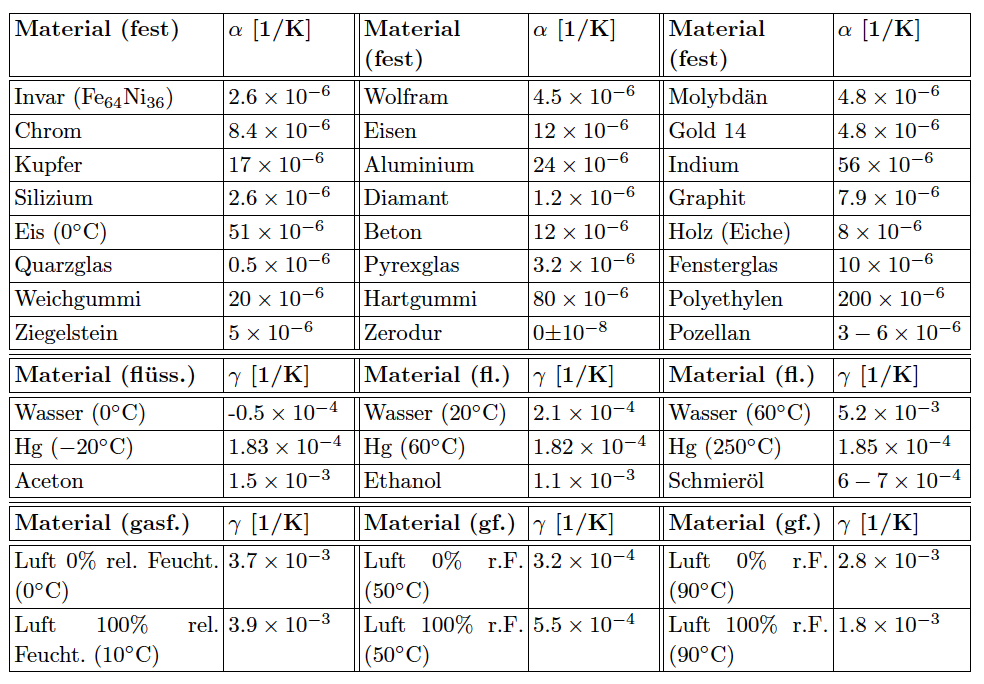
\includegraphics[scale=0.6]{../img/I/Id}}
\centering
\caption{Ausdehnungskoeffizienten einiger Materialien bei 1 bar Umgebungsdruck.}
\label{fig_Id}
\end{figure}
\noindent Im allgemeinen dehnt sich ein Körper aus, wenn er erwärmt wird. Tritt bei der Erwärmung keine chemische oder strukturelle Änderung des Körpers auf, so erfolgt die \textbf{Dehnung} näherungsweise proportional zur Temperaturänderung. 
\\\\
Ändert sich die Temperatur eines Stabes mit Länge $l_0$ um die Grösse $\triangle \theta$, so erfährt dieser eine \textbf{Längenänderung} $\triangle l$, welche näherungsweise proportional zur Temperaturänderung $\triangle \theta$ ist, wobei $\alpha$ der \textbf{Längenausdehnungskoeffizient} mit Einheit K$^{-1}$.
\begin{equation}
\boxed{\triangle l\approx \alpha\cdot l_0\cdot \triangle \theta}
\end{equation}
Ändert sich die Temperatur eines Körpers mit Volumen $V_0$ um die Grösse $\triangle \theta$, so erfährt dieser eine \textbf{Volumenänderung} $\triangle l$, welche näherungsweise proportional zur Temperaturänderung $\triangle \theta$ ist, wobei $\gamma$ der \textbf{Volumenausdehnungskoeffizient} mit Einheit K$^{-1}$.
\begin{equation}
\boxed{\triangle V\approx \gamma\cdot V_0\cdot \triangle \theta}
\end{equation}
Da $\alpha$ und $\gamma$ im allgemeinen temperaturabhängige Grössen sind, werden die Beziehungen für den allgemeinen Fall, im welchem die Beziehung zwischen Ausdehnung und Temperatur nicht linear verläuft, in \textbf{Differentiation} geschrieben.
\begin{equation}
\boxed{\dfrac{\text{d}}{\text{d}\theta}\Big[l\left(\theta\right)\Big]=\alpha\left(\theta\right)\cdot l\left(\theta\right)}\quad \boxed{\dfrac{\text{d}}{\text{d}\theta}\Big[V\left(\theta\right)\Big]=\gamma\left(\theta\right)\cdot V\left(\theta\right)}
\end{equation}
Für \textbf{isotrope Körper}, d.h. Körper, deren physikalische Eigenschaften richtungsunabhängig sind gilt
\begin{equation}
\boxed{\gamma=3\cdot \alpha}
\end{equation}
\subsection{Die Anomalie des Wassers}
\begin{figure}[H]
\frame{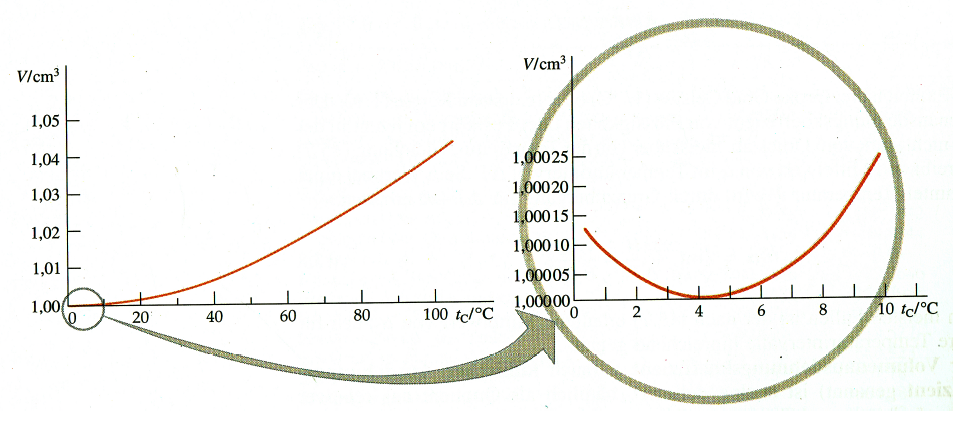
\includegraphics[scale=0.6]{../img/I/Ie}}
\frame{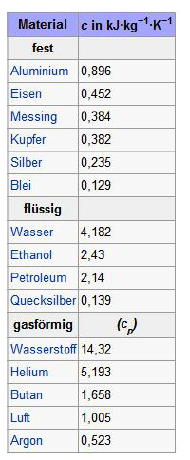
\includegraphics[scale=0.6]{../img/I/If}}
\centering
\caption{Volumen von 1g Wasser in Abhängigkeit der Tempeartur.}
\label{fig_Ie}
\end{figure}
Die meisten Substanzen dehnen sich beim Aufwärmen aus. Eine wichtige Ausnahme davon ist Wasser, dessen Volumen im Bereich zwischen 0$^{\circ}$C und 4$^{\circ}$C mit zunehmender Temperatur kleiner wird. Die Funktion $V\left(^{\circ}C\right)$ hat einen Minimum bei $4^{\circ}$C. Wasser besitzt bei 4$^{\circ}$C die grösste Dichte. Wird im Winter das Wasser eines Sees durch die kalte Umgebungsluft abgekühlt, so nimmt die Dichte des Wassers zu, und es sinkt nach unten. Unterhalb von 4$^\circ$C die Wasserdichte wieder abnimmt, sammelt sich Wasser mit Temperaturen kleiner als 4$^\circ$C an der Wasseroberfläche an.
\\\\
Dies führt dazu, dass allfällige Frostbildung im See an der Oberfläche stattfindet, und sich Wasser mit 4$^\circ$C Temperatur dann am Seeboden ansammelt. Weil die Dichte von Eis kleiner als jene von Wasser ist, bleibt das Eis oben und sinkt nicht zum Grund.
\subsection{Die spezifische Wärmekapazität}
Nimmt der Körper Wärme auf oder gibt er Wärme ab, so kann sich seine Temperatur ändern. Damit lässt sich die Fähigkeit von Materie, Energie zu speichern in Zusammenhang mit Temperaturänderungen der Materie bringen. Die Wärmemenge $\triangle Q$, die benötigt wird, um einen Körper um eine bestimmte Temperatur zu erwärmen hängt ab von der \textbf{Masse} des Körpers und von der \textbf{Fähigkeit} des Materials, aus welchem der Körper besteht, Wärme zu speichern. Die \textbf{spezifische Wärmekapazität} als Wärmemenge die benötigt wird, um 1kg eines Stoffes um 1K zu erwärmen.
\begin{equation}
\boxed{c=\dfrac{\triangle Q}{m\cdot \triangle \theta},\quad [c]=\text{J}\,\text{kg}^{-1}\,\text{K}^{-1}}
\end{equation}
Dabei ist $\triangle Q$ die thermische Energie, die der Materie zugeführt oder entzogen wird, $m$ ist die Masse der Substanz, $c$ ist die spezifische Wärmekapazität und $\triangle \theta$ ist die Temperaturänderung.
\subsection{Phasenumwandlungen und latente Wärme}
\begin{figure}[H]
\frame{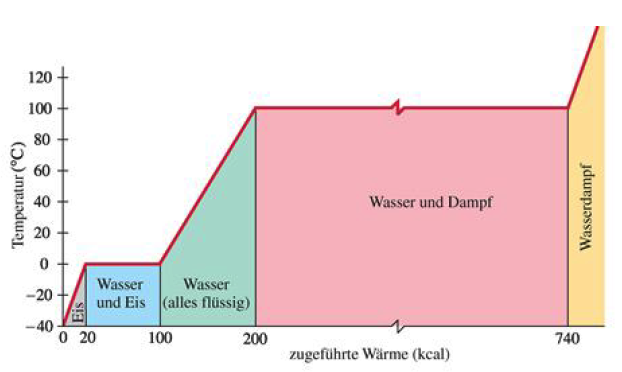
\includegraphics[scale=0.6]{../img/I/Ig}}
\centering
\caption{Temperatur als Funktion der zugeführten Wärme, die 1kg Eis bei $-40^{\circ}$C in über $100^{\circ}$C heissen Dampf verwandelt. Zu beachten ist den Skalenbruch zwischen 200 und 740kcal.}
\label{fig_Ig}
\end{figure}
Wird trotz Wärmezufuhr oder -abfuhr keine Temperaturänderung gemessen, so findet im betroffenen Material eine \textbf{Phasenumwandlung} statt.
\begin{enumerate}
\item \textbf{Schmelzen:} Von fest zu flüssig.
\item \textbf{Verdampfen:} Von flüssig zu gasförmig.
\item \textbf{Sublimieren:} Von fest zu gasförmig.
\item \textbf{Erstarren:} Von flüssig zu fest.
\item \textbf{Kondensieren:} Von gasförmig zu flüssig oder fest.
\end{enumerate}
Eine Temperaturänderung hängt mit der Änderung der kinetischen Energie der Teilchen des Körpers zusammen. Bei einer Phasenumwandlung ändern sich die Bindungszustände und somit die potentielle Energie der Teilchen im Körper.
\\\\
Um einen festen Körper zu schmelzen, muss man eine materialspezifische Energiemenge aufwenden, die sogenannte Schmelzwärme. Beim Gefrieren bzw. Erstarren wird diese Energie wieder freigesetzt. Das Gleiche gilt für die Verdampfung und Kondensation. Da die Verdampfungswärme oft einer verdunstenden Flüssigkeit entzogen wird, nennt man sie auch Verdunstungskälte, da die verbleibende Flüssigkeit kälter wird. Da sich beim Phasenübergang die Temperatur durch Wärmezufuhr nicht ändert, wird die für den Phasenübergang notwendige Wärme auch \textbf{latente Wärme} genannt. 
\\\\
Unter der \textbf{spezifischen Schmelzwärme} $q_s$ versteht man die Energie, die benötigt wird, um 1kg einer Materie aus dem festen in den flüssigen Aggregatzustand zu versetzen.
\begin{equation}
\boxed{\triangle Q=q_s\cdot m,\quad [\triangle Q]=\text{J},\quad q_{s,H_2O}=333.5\text{kJ kg}^{-1}}
\end{equation}
Die \textbf{spezifische Verdampfungswärme} $q_v$ ist die Energiemenge, die benötigt wird um 1kg einer Flüssigkeit am Siedepunkt vollständig zu verdampfen.
\begin{equation}
\boxed{\triangle Q=q_v\cdot m,\quad [\triangle Q]=\text{J},\quad q_{v,H_2O}=2250\text{kJ kg}^{-1}}
\end{equation}
\subsection{Temperaturausgleich und Mischtemperaturen}
Bei Temperaturausgleichen zwischen zwei Stoffen wird Wärmeenergie von einem Stoff abgegeben und vom anderen aufgenommen, bis das thermische Gleichgewicht bei der Mischtemperatur $\theta_M$ erreicht ist. Falls keine Phasenumwandlungen stattfinden, ergibt sich die Energiebilanz
\begin{equation}
\boxed{\triangle E=\triangle Q=\displaystyle \sum_{i}^n\Big[c_i\cdot m_i\cdot \left(\theta_M-\theta_i\right)\Big]=0}
\end{equation}
\subsection{Der erste Hauptsatz der Thermodynamik}
Wird einer Substanz Wärme zugeführt, so wird diese in Materie gespeichert. Es kommen drei Formen von Energien vor: die \textbf{kinetische}, die \textbf{potentielle} und die \textbf{chemische Energie}. Die Summe aller in der Materie gespeicherte Energie wird als \textbf{innere Energie} $U$ bezeichnet.
\\\\
Ein \textbf{geschlossenes System} kann mit seiner Umgebung Energie in Form von Wärme $Q$ und Arbeit $W$ austauschen. $U$ ist eine \textbf{Zustandsgrösse} oder \textbf{Zustandsgrösse} und $Q$ und $W$ sind Die Änderung der inneren Energie $\text{d}U$ eines geschlossenen Systems ergibt sich aus der Summe der ausgetauschten Wärme und der verrichtete Arbeit
\begin{equation} 
\boxed{\text{d}U=\delta Q+\delta W,\quad [\text{d}U]=\text{J}}
\end{equation} 
Im stationären Zustand, d.h. wenn sich die innere Energie nicht ändert und für die Leistung gilt
\begin{equation}
\boxed{\delta Q+\delta W=0}\quad \boxed{\delta \dot{Q}+\delta \dot{W}=0}
\end{equation}
\subsection{Wärmeübertragung}
Steht ein Körper in thermischen Kontakt mit seiner Umgebung, wird Wärme übertragen, wenn zwischen dem Körper und seiner Umgebung eine \textbf{Temperaturdifferenz} besteht. Diese Wärmeübertragung geht immer vom Körper mit der höheren Temperatur zum Körper mit der tieferen Temperatur. Der umgekehrte Vorgang findet spontan nicht statt. Die Wärmeübertragung ist für die Energietechnik von grosser Bedeutung.
\\\\
Wärme kann durch drei verschiedene physikalische Prozesse übertragen werden: durch \textbf{Wärmeleitung}, durch \textbf{Konvenktion} und durch \textbf{elektromagnetische Strahlung}.
\subsection{Wärmeleitung}
Der Wärmestrom fliesst von den Stellen mit höherer Temperatur zu den Stellen mit tieferer Temperatur eines Körpers. Dadurch nimmt die Temperatur an den Quellen des Wärmestroms ab und an den Senken zu. Dieser Wärmestrom fliesst solange, bis sich die Temperaturen im ganzen Körper ausgeglichen haben und der Körper im thermischen Gleichgewicht ist. Wird eine konstante Temperaturdifferenz aufrecht erhalten, so stellt sich ein \textbf{stationärer Zustand} ein. 
\\\\
Stellt man sich die Wärme als kinetische Schwingungsenergie der atomaren elementaren Bestandteile der Materie vor, so schwingen die Teile höherer Temperatur stärker und geben über Stösse ihre Energie teilweise an die Nachbarn weiter. So verteilt sich diese kinetische Energie im ganzen Körper, bis er entweder im thermischen Gleichgewicht oder im stationären Zustand ist.
\subsubsection{Wärmeleitung durch eine einschichtige Wand}
\begin{figure}[H]
\frame{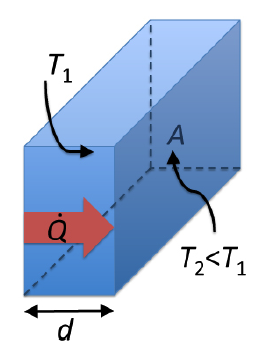
\includegraphics[scale=0.5]{../img/I/Ih}}
\centering
\caption{Wärmeleitung durch eunen Quader mit Seitenlänge $A$ und Dicke $d$. Der Wärmefluss wird durch den Temperaturunterschied verursacht.}
\label{fig_Ih}
\end{figure}
Die Wärmeleitung durch eine einschichtige Wand mit einer Fläche $A$ mit Dicke $d$ mit Temperaturen $\theta_1$ und $\theta_2$, mit $\theta_2<\theta_1$, lässt sich der \textbf{Wärmestrom} $\dot{Q}$, wobei $\lambda$ eine Materialgrösse ist und heisst \textbf{Wärmeleitungskoeffizient} $[\lambda]=\text{Watt m}^{-1} \text{K}^{-1}$, bestimmen. Der Wärmestrom ist also umso grösser, je grösser die Temperaturdifferenz $\triangle \theta = \theta_1-\theta_2$ als treibende Kraft und die Kontaktfläche $A$, und umso kleiner, je grösser der Weg $d$ ist.
\begin{equation}
\boxed{\dot{Q}=\dfrac{\triangle \theta}{R_{\text{th}}}=\dfrac{\lambda\cdot A}{d}\cdot \left(\theta_1-\theta_2\right),\quad [\dot{Q}]=\text{J s}^{-1}=\text{Watt}}\quad \boxed{R_{\text{th}}=\dfrac{d}{\lambda\cdot A},\quad [R_{\text{th}}]=\text{K Watt}^{-1}}
\end{equation}
Der \textbf{thermische Widerstand} $R_{\text{th}}$, in Analogie zum elektrischen Widerstand $R_{\text{el}}=\dfrac{l}{\sigma\cdot A}$, gibt an, welche Temperaturdifferenz notwendig ist, um einen Wärmestrom von 1Watt durch eine ebene Wand zu erzeugen. Die Dicke der Wand ist im thermischen Widerstand bereits eingerechnet.
\subsubsection{Wärmeleitung durch eine mehrschichtige Wand}
\begin{figure}[H]
\frame{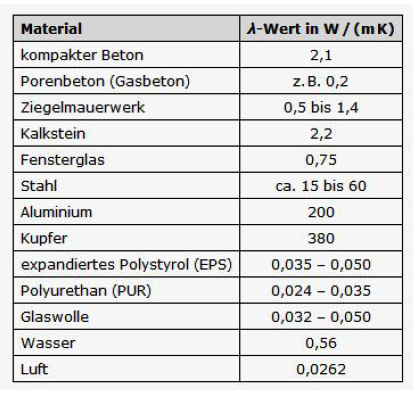
\includegraphics[scale=0.7]{../img/I/Ij}}
\frame{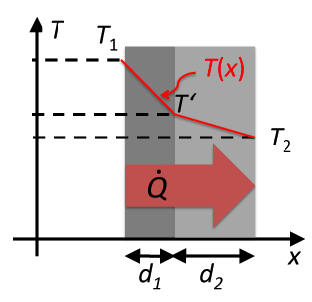
\includegraphics[scale=0.7]{../img/I/Ik}}
\centering
\caption{\textbf{\textit{Links:}} Wärmeleitfähigkeit ausgewählter Materialien. \textbf{\textit{Rechts:}} Temperaturverlauf bei der Wärmeleitung einer mehrschichtige Wand.}
\label{fig_Ij}
\end{figure} 
Werden mehrere homogene Schichten von Materialien aneinander gereiht, so addieren sich die thermischen Widerstände, äquivalent zur Serienschaltung elektrischer Netzwerke.
\begin{equation}
\boxed{R_{\text{th, tot}}=R_{\text{th, 1}}+R_{\text{th, 2}}+\dotso+R_{\text{th, n}}=\dfrac{1}{A}\cdot \left(\dfrac{d_1}{\lambda_1}+\dfrac{d_2}{\lambda_2}+\dotso+\dfrac{d_n}{\lambda_n}\right)}
\end{equation}
Im stationären Fall ist der Wärmestrom durch jede Schicht gleich gross
\begin{equation}
\boxed{\dot{Q}_1=\dot{Q}_2=\dotso=\dot{Q}_n}
\end{equation}
Der Wärmestrom durch einemehrschichtige Wand lautet
\begin{equation}
\boxed{\dot{Q}_{\text{tot}}=\dfrac{\triangle \theta_{\text{tot}}}{R_{\text{th, tot}}}}
\end{equation}
Die Zwischentemperatur lautet
\begin{equation}
\boxed{\theta'=\theta_1-\dot{Q}\cdot R_{\text{th, 1}}=\theta_2-\dot{Q}\cdot R_{\text{th, 2}}}
\end{equation}
\subsubsection{Wärmeleitung durch ein Rohr}
\begin{figure}[H]
\frame{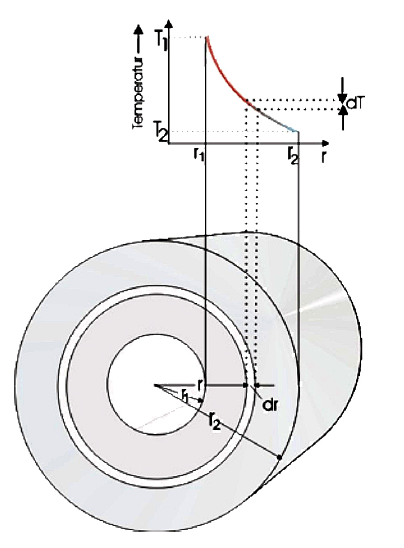
\includegraphics[scale=0.7]{../img/I/Il}}
\centering
\caption{Wärmeleitung durch ein Rohr. Die Temperaturabfall wird über eine infinitesimal dicke Schicht und dann über die Rohrdicke integriert.}
\label{fig_Il}
\end{figure} 
Denkt man sich ein zylindrisches Rohr in konzentrische dünne Schichten zerlegt, so erkennt man, dass der thermische Widerstand der einzelnen Schichten gegen aussen kleiner wird, weil die Fläche zunimmt. Entsprechend ergibt sich in der Wand kein linearer Temperaturverlauf mehr. Betrachte man ein Zylinder der Länge $l$, Innenradius $r_1$ und Aussenradius $r_2$. Die Temperaturen an der Innen- und Aussenseite des Zylinders betragen $\theta_1$ und $\theta_2>\theta_1$. Für den Temperaturverlauf $\text{d}\theta$ über eine infinitesimal dünne Scheibe des Zylinders der Dicke $\text{d}r$ mit Radius $r$ und Fläche $A=2\pi r l$ gilt
\begin{equation}  
\boxed{
\begin{array}{lll}
\text{d}\theta&=&\dot{Q}\cdot \text{d}R_{\text{th}}=\dot{Q}\cdot \dfrac{\text{d}r}{\lambda\cdot A}=\dot{Q}\cdot \dfrac{\text{d}r}{\lambda\cdot 2\pi\cdot r\cdot l}
\\
\displaystyle\int_{\theta_1}^{\theta_2}\text{d}\theta&=&\displaystyle\int_{r_1}^{r_2}\dot{Q}\cdot \dfrac{\text{d}r}{\lambda\cdot 2\pi\cdot r\cdot l}
\\
\theta_2-\theta_1&=&\dot{Q}\cdot \dfrac{\ln\left(r_2\right)-\ln\left(r_1\right)}{\lambda\cdot 2\pi\cdot l}=\dfrac{\dot{Q}}{\lambda\cdot 2\pi\cdot l}\cdot \ln\left(\dfrac{r_2}{r_1}\right)
\\
\end{array}
}
\end{equation} 
Die Reihenfolge der Integrationsgrenzen sind so gesetzt, dass der Wärmestrom von aussen nach innen ein positives Vorzeichen hat. Aufgelöst nach dem Wärmestrom ergibt
\begin{equation}
\boxed{\dot{Q}=\dfrac{\lambda\cdot 2\pi\cdot l}{\ln\left(r_2/r_1\right)}\cdot \left(\theta_2-\theta_1\right)}  
\end{equation}  
Für den thermischen Widerstand ergibt sich
\begin{equation}
\boxed{R_{\text{th}}=\dfrac{1}{2\pi\cdot \lambda\cdot l}\cdot \ln\left(\dfrac{r_2}{r_1}\right)} 
\end{equation}  
Fliesst die Wärme von aussen nach innen $\left(\theta_2>\theta_1\right)$ so gilt $\dot{Q}>0$. Der Temperaturverlauf lautet
\begin{equation}
\boxed{\theta\left(r\right)=\theta_2-\dot{Q}\cdot \dfrac{\ln\left(r/r_1\right)}{\lambda\cdot 2\pi\cdot l}}  
\end{equation}  
\subsection{Konvenktion}
Konvenktion ist das Mitführen von thermischer Energie (innerer Energie) in strömenden Fluiden (Flüssigkeiten oder Gasen). Bei Konvektion bewegen sich die Teilchen eines Fluids durch den Raum und transportieren dabei Wärmeenergie. Konvenktion ist an \textbf{Materie} verbunden. Der Transport von Wärme über Konvenktion ist grösser als über Wärmeleitung.
\\\\
\textbf{Freier Konvektion:} Der Strömungsprozess entsteht wegen örtlicher Unterschiede in der Dichte. Wird ein Fluid erwärmt, so dehnt sich aus und damit nimmt seine Dichte ab. Liegt ein Fluid mit geringerer Dichte unter einem Fluid mit höherer Dichte, steigt der erwärmte Stoff infolge des Auftriebs nach oben. Es bildet sich eine Strömung aus.
\\\\
\textbf{Erzwungener Konvenktion:} Bei der erzwungener Konvenktion wird die Strömung mittels Pumpen oder Ventilatoren erzwungen.
\subsection{Wärmestrom durch Konvenktion}
Stehen eine warme Fläche und ein kühleres Medium im Kontakt, bildet sich entlang dem Körper eine Grenzschicht aus: Das strömende Medium hat unmittelbar an der Wand die Strömungsgeschwindigkeit 0 und die Temperatur der Wand, mit zunehmender Distanz von der Wand steigt die Strömungsgeschwindigkeit an auf $u_{\infty}$, während gleichzeitig die Temperatur abnimmt auf einen Wert $\theta_{\infty}$, der Mediumstemperatur weit weg von der Wand.
\\\\
Der Wärmeübergang durch Konvenktion kann mit Hilfe eines thermischen Widerstandes dargestellt werden, wobei $h$ der Wärmeübergangskoeffizient, eine gekoppelte Strömung destransportierenden Fluids, $A$ die Fläche und $\theta_{\infty}$ die Temperatur ausserhalb der Grenzschicht.
\begin{equation}
\boxed{\dot{Q}=\dfrac{\theta_{\text{Wand}}-\theta_{\infty}}{R_{\text{th}}}=h\cdot A\cdot \left(\theta_{\text{Wand}}-\theta_{\infty}\right),\quad [h]=\text{Watt m}^{-2}\text{K}^{-1}}\quad \boxed{R_{\text{th}}=\dfrac{1}{h\cdot A}}
\end{equation}
\begin{figure}[H]
\frame{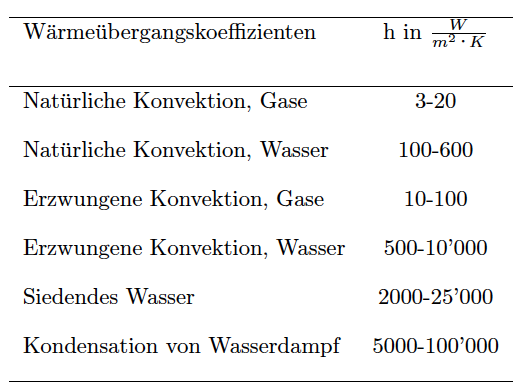
\includegraphics[scale=0.6]{../img/I/Im}}
\centering
\caption{Wärmeübergangskoeffizienten.}
\label{fig_Im}
\end{figure}
\subsection{Wärmeübertrager}
\textbf{Wärmeübertrager} sind wichtige Elemente der Energietechnik, die im Wesentlichen auf \textbf{Konvenktion} beruhen. Zwei Fluide unterschiedlicher Temperatur werden über eine grosse Oberfläche in thermischen Kontakt gebracht, mit dem Ziel, Wärmeenergie aus dem heisseren Fluid aufs kältere Fluid zu übertragen. Für einen effizienten Wärmeaustausch soll der thermische Widerstand zwischen den Fluiden möglichst gering sein. Dazu sind auch hohe Wärmeübergangskoeffizienten zwischen den Fluiden und der umliegenden Oberfläche notwendig. Eine Anwendung ist die Komfortluftung in einem modernen Minergie-Gebäude: Die Frischluft wird über einen Wärmeübertrager von der verbrauchten Abluft erwärmt und so der Energieverlust durch die Luftung erheblich reduziert.
\begin{figure}[H]
\frame{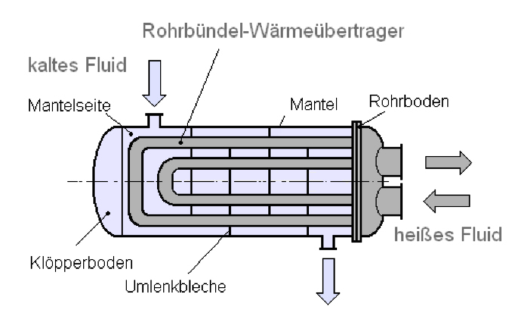
\includegraphics[scale=0.7]{../img/I/In}}
\centering
\caption{SchematischeIllustration eines Wärmetauschers.}
\label{fig_In}
\end{figure}
\subsection{Wärmedurchgang}
Als \textbf{Wärmeübergang} versteht man die Wärmeübertragung von einem Fluid durch eine Wand auf ein anderes Fluid. Die Wärme aus dem Fluid geht dabei durch Konvenktion über auf die Wand, mit Wärmeleitung durch die Wand und schliesslich wieder durch Konvenktion ins kältere Fluid über.
\begin{figure}[H]
\frame{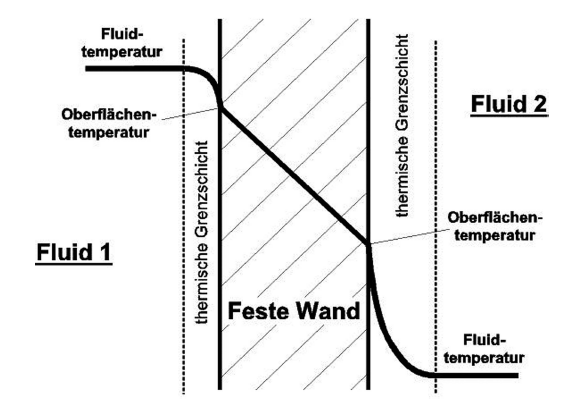
\includegraphics[scale=0.6]{../img/I/Io}}
\centering
\caption{Wärmefluss durch eine Wand unter Berücksichtigung des Wärmeübergangs ander Wandoberfläche zu den angrenzenden Fluiden.}
\label{fig_Io}
\end{figure}
\noindent Den gesamten Wärmedurchgang eines Schichtsystems mit konstanter Fläche $A$ beschreibt man mittels des U-Werts
\begin{equation}
\boxed{\dot{Q}=U\cdot A\cdot\left(\theta_2-\theta_1\right),\quad [U]=\text{Watt m}^{-2}\text{K}^{-1}}
\end{equation}
Für die Berechnung des $U$-Wertes verwendet man wieder das Konzept des thermischen Widerstands.
\begin{equation}
\boxed{U=\dfrac{1}{R_{\text{th, tot}}\cdot A}}
\end{equation}
Der gesamte thermische Widerstand $R_{\text{th, tot}}$ setzt sich zusammen aus den konvenktiven Widerständen auf der Innen- und Aussenseite und aus dem thermischen Widerstand der Wand, wobei $h_i$ und $h_a$ die Wärmeübergangskoeffizienten innen und aussen und $d_j$ und $\lambda_j$ die Wärmeleitkoeffizienten der einzelnen Wandschichten sind.
\begin{equation}
\boxed{R_{\text{th, tot}}=R_{\text{th, i}}+R_{\text{th, W}}+R_{\text{th, a}}}
\end{equation}
\begin{equation}
\boxed{U=\left(\dfrac{1}{h_i}+\dfrac{d_1}{\lambda_1}+\dfrac{d_2}{\lambda_2}+\dotso+\dfrac{d_n}{\lambda_n}+\dfrac{1}{h_a}\right)^{-1},\quad [U]=\text{Watt m}^{-2}\text{ K}^{-1}}
\end{equation}
Kennt man den Wärmestrom, so lassen sich daraus auch die Temperaturen der Wandoberfläche berechnen: Die Temperaturänderung ergibt sich aus dem thermischen Widerstand. Geht man von einer Aussentemperatur und eine Innentemperatur und verwendet man die konvenktiven thermischen Widerstände auf der Innen- und auf der Aussenseite, findet man
\begin{equation}
\boxed{\theta_{W,i}=\theta_{\infty, i}-\dfrac{\dot{Q}}{h_i\cdot A_i}}\quad \boxed{\theta_{W,a}=\theta_{\infty, a}-\dfrac{\dot{Q}}{h_a\cdot A_a}}
\end{equation}
Die Innentemperatur mit zunehmender Dämmschicht nähert der Raumtemperatur an, was eine deutliche Komfortsteigerung bedeutet.
\begin{figure}[H]
\frame{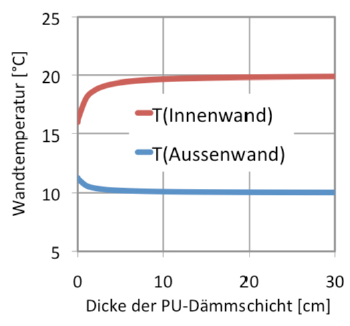
\includegraphics[scale=0.7]{../img/I/Ip}}
\centering
\caption{Einfluss der Dicke der Dämmschicht auf die Temperaturen direkt auf der Wand (innnen und aussen).}
\label{fig_Ip}
\end{figure}
\subsection{Luftfeuchtigkeit und der Taupunkt}
Die Umgebungsluft enthält immer auch eine gewisse Menge Wasserdampf,welcher unter bestimmten Bedingungen kondensieren kann. Bei vielen Baustoffen kann die Wärmeleitfähigkeit erheblich ansteigen, wenn Feuchtigkeit auftritt. Kondensation an Innenwänden, aber auch in Zwischenräumen kann aber auch zu Schimmelbildung und Schäden an den Bausubstanz führen. Die Masse an Wasserdampf, die ein bestimmtes Luftvolumen enthalten kann ist abhängig von der Temperatur. 
\\\\
Man unterscheidet zwischen der \textbf{absoluten Luftfeuchtigkeit}, d.h. die in einem bestimmten Luftvolumen erhaltene Wasserdampfmasse $m_w$ 
\begin{equation}
\boxed{f=\dfrac{m_w}{V},\quad [f]=\text{g m}^{-3}}
\end{equation}
und der \textbf{relativen Luftfeuchtigkeit}, d.h. das Verhältnis zwischen absoluter Luftfeuchtigkeit und maximaler Luftfeuchtigkeit bei gegebener Temperatur.
\begin{equation}
\boxed{\phi=\dfrac{f}{f_{\text{max}}}\cdot 100\%}
\end{equation}
Wird $f_{\text{max}}$ erreicht, so ist die Luft gesättigt und der Wasserdampf kondensiert. Die entsprechende Temperatur wird als \textbf{Taupunkt} bezeichnet.
\newline\newline
Bei der Planung einer Gebäudekonstruktion müssen also nicht nur der U-Wert, sondern auch die Zwischentemperaturen in der Wand und der Taupunkt berücksichtigt werden. Dabei soll der Taupunkt so weit aussen wie möglich zu liegen kommen.
\begin{figure}[H]
\frame{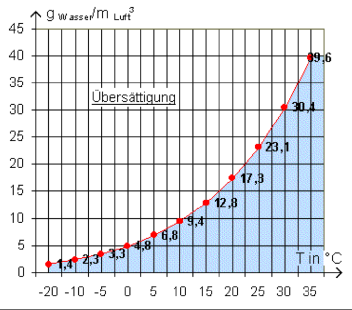
\includegraphics[scale=0.7]{../img/I/Iq}}
\centering
\caption{Taupunkte für Wasserdampf in Luft. Die rote Linie gibt die Masse an Wasserdampf für welche eine relative Luftfeuchte von 100\% erreicht wird.}
\label{fig_Iq}
\end{figure}
\begin{figure}[H]
\frame{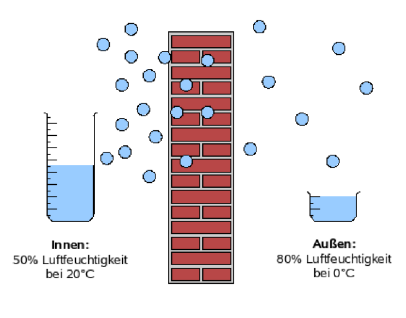
\includegraphics[scale=0.7]{../img/I/Ir}}
\centering
\caption{Unter der Annahme, dass die absolute Luftfeuchtigkeit innen und aussen gleich ist, ändert sich die relative Luftfeuchtigkeit als Funktion der Temperatur über der Wand.}
\label{fig_Ir}
\end{figure}




















